% Options for packages loaded elsewhere
\PassOptionsToPackage{unicode}{hyperref}
\PassOptionsToPackage{hyphens}{url}
%
\documentclass[
]{article}
\usepackage{amsmath,amssymb}
\usepackage{iftex}
\ifPDFTeX
  \usepackage[T1]{fontenc}
  \usepackage[utf8]{inputenc}
  \usepackage{textcomp} % provide euro and other symbols
\else % if luatex or xetex
  \usepackage{unicode-math} % this also loads fontspec
  \defaultfontfeatures{Scale=MatchLowercase}
  \defaultfontfeatures[\rmfamily]{Ligatures=TeX,Scale=1}
\fi
\usepackage{lmodern}
\ifPDFTeX\else
  % xetex/luatex font selection
\fi
% Use upquote if available, for straight quotes in verbatim environments
\IfFileExists{upquote.sty}{\usepackage{upquote}}{}
\IfFileExists{microtype.sty}{% use microtype if available
  \usepackage[]{microtype}
  \UseMicrotypeSet[protrusion]{basicmath} % disable protrusion for tt fonts
}{}
\makeatletter
\@ifundefined{KOMAClassName}{% if non-KOMA class
  \IfFileExists{parskip.sty}{%
    \usepackage{parskip}
  }{% else
    \setlength{\parindent}{0pt}
    \setlength{\parskip}{6pt plus 2pt minus 1pt}}
}{% if KOMA class
  \KOMAoptions{parskip=half}}
\makeatother
\usepackage{xcolor}
\setlength{\emergencystretch}{3em} % prevent overfull lines
\providecommand{\tightlist}{%
  \setlength{\itemsep}{0pt}\setlength{\parskip}{0pt}}
\setcounter{secnumdepth}{-\maxdimen} % remove section numbering
\ifLuaTeX
  \usepackage{selnolig}  % disable illegal ligatures
\fi
\IfFileExists{bookmark.sty}{\usepackage{bookmark}}{\usepackage{hyperref}}
\IfFileExists{xurl.sty}{\usepackage{xurl}}{} % add URL line breaks if available
\urlstyle{same}
\hypersetup{
  hidelinks,
  pdfcreator={LaTeX via pandoc}}

\author{}
\date{}

\begin{document}

This is some text \textless-extracted text-\textgreater{} in between the
delimiters now the second line --- title: Just say hello! author: My
Friend header-includes: \textbar{}

\usepackage{tikz,pgfplots}
    \usepackage{fancyhdr}
    \pagestyle{fancy}
    \fancyhead[CO,CE]{This is fancy}
    \fancyfoot[CO,CE]{So is this}
    \fancyfoot[LE,RO]{\thepage}

\hypertarget{abstract-this-is-a-pandoc-test-with-markdown-inline-latex}{%
\subsection{abstract: This is a pandoc test with Markdown + inline
LaTeX}\label{abstract-this-is-a-pandoc-test-with-markdown-inline-latex}}

\hypertarget{just-say-hello}{%
\section{Just say hello!}\label{just-say-hello}}

This could be a good example or inlined \LaTeX:

\begin{tikzpicture}
\begin{axis}
\addplot[color=red]{exp(x)};
\end{axis}
\end{tikzpicture}

\%Here ends the furst plot \hskip 5pt \%Here begins the 3d plot

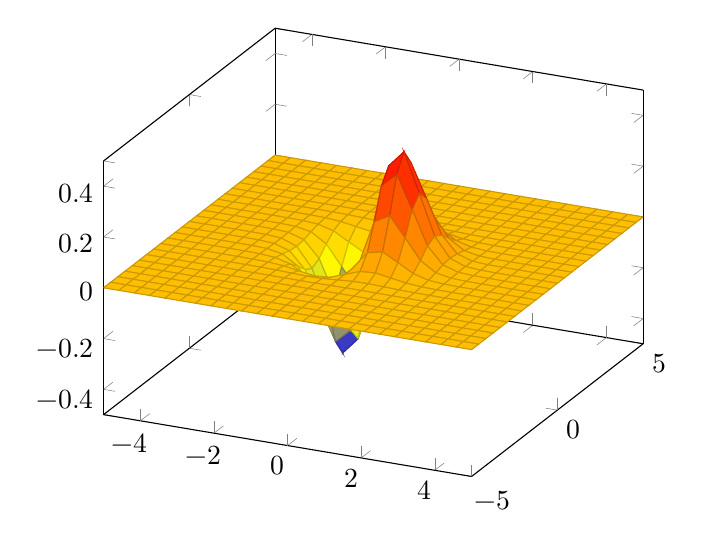
\begin{tikzpicture}
\begin{axis}
\addplot3[
    surf,
]
{exp(-x^2-y^2)*x};
\end{axis}
\end{tikzpicture}

And now, just a few words to terminate:

\begin{quote}
Goodbye folks!
\end{quote}

Which can be converted to LaTeX using commands like this: pandoc -s -i
pretty\_md\_test.md -o pretty\_md\_test.tex

the thirdline \textless-fig1-\textgreater{} further
\textless-fig1-code-\textgreater{} \textless-table1-code-\textgreater{}
text insert a string in the text \textless-str1-code-\textgreater{} and
now

\end{document}
